\chapter{ Data processing}
\section{kNN}
The dataprocessing will consist of finding the optimal k and smoothing and DPI which lowers the error rate  This is found by applying knn on different training set, with different smoothing levels, and DPI.  For each case will an contour plot be made, which shows that how each parameter effect each other, and thereby be useful for deciding which parameter gives the optimal peformance. \\

Different smoothing techniques were applied to the images, such as Gaussian blur and average filters.  
For each were knn applied with different values of, and for each were error rate computed.  Thereby would it be possible to find the optimal parameter for this sort of problem, considering the smoothing and value of k. 


\begin{figure}[H]    
	\begin{minipage}[t]{0.45\textwidth}
		\centering
			
\includegraphics[width=0.4\linewidth]{figure/mikael_8_2_dpi100_k3.png}
			\caption{DPI = 100 , kernel size = 3}
			\label{fig:dpi_100_3}
	\end{minipage}
	\hspace{\fill}
	\begin{minipage}[t]{0.45\textwidth}
		\centering
			
\includegraphics[width=0.4\linewidth]{figure/mikael_8_2_dpi100_k5.png}
			\caption{DPI = 100 , kernel size = 5}
			\label{fig:dpi_100_5}
	\end{minipage}

\vspace*{0.5cm} % (or whatever vertical separation you prefer)
	\begin{minipage}[t]{0.45\textwidth}
		\centering
			
\includegraphics[width=0.4\linewidth]{figure/mikael_8_2_dpi300_k5.png}
			\caption{DPI = 300 , kernel size = 5}
			\label{fig:dpi_300_5}
	\end{minipage}
\hspace{\fill}
	\begin{minipage}[t]{0.45\textwidth}
		\centering
			
\includegraphics[width=0.4\linewidth]{figure/mikael_8_2_dpi300_k9.png}
			\caption{DPI = 300 , kernel size = 9}
			\label{fig:dpi_300_9}
	\end{minipage}
\caption{Effect of smoothing using average filter with different kernel sizes}
\end{figure}

\begin{figure}[H]
\centering
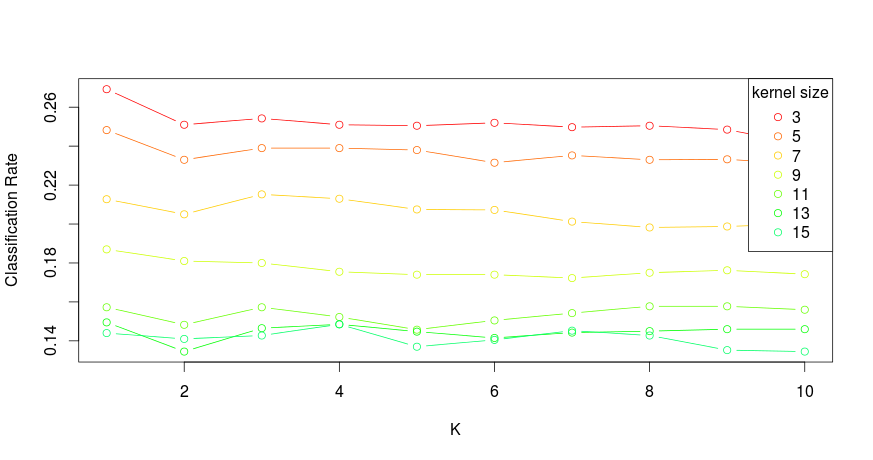
\includegraphics[width = \textwidth]{figure/data_100_15_10.png}
\caption{Tested on images with 100 dpi}
\label{fig:data_100}
\end{figure}

\begin{figure}[H]
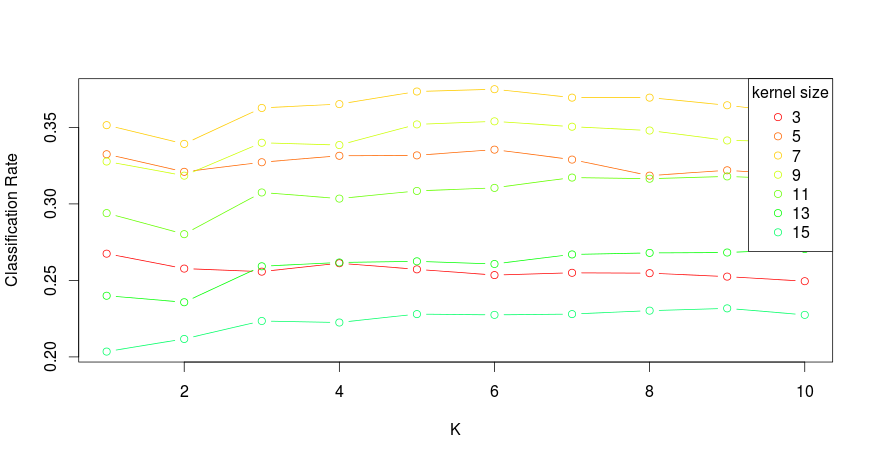
\includegraphics[width = \textwidth]{figure/data_200_15_10.png}
\caption{Tested on images with 200 dpi}
\label{fig:data_200}
\end{figure}

\begin{figure}[H]
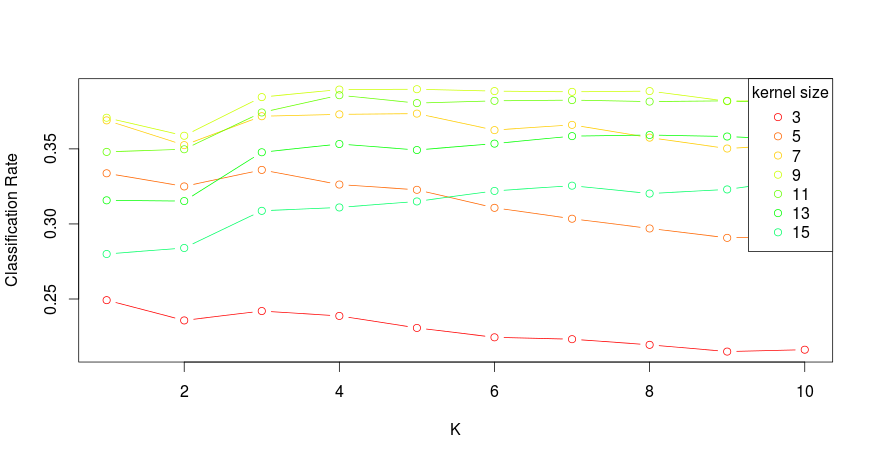
\includegraphics[width = \textwidth]{figure/data_300_15_10.png}
\caption{Tested on images with 300 dpi}
\label{data_300}
\end{figure}
\missingfigure{Knn-  smooth Gaussian images. }
\missingfigure{Knn-  smooth Gaussian images plots }